\section{Calibration} \label{sec:calib}

In this section the various calibration procedures taken in order to minimize the time resolution and enhance both the particle identification (PID) and time of flight (TOF) capabilities of the Start Counter are discussed.

\subsection{Time-Walk Correction} \label{sec:calib_tw}

The time-walk effect is a well understood consequence of leading edge discriminators (LED).  Analog signals of varying amplitudes crossing a fixed threshold, as determined by the discriminator threshold setting, will do so at varying times.

The time-walk effect is attributed to larger signals having faster rise times as compared to signals which have amplitudes close to the threshold setting, see Fig.~\ref{fig:time_walk_effect}.
\begin{figure}[!htb]
	\centering
	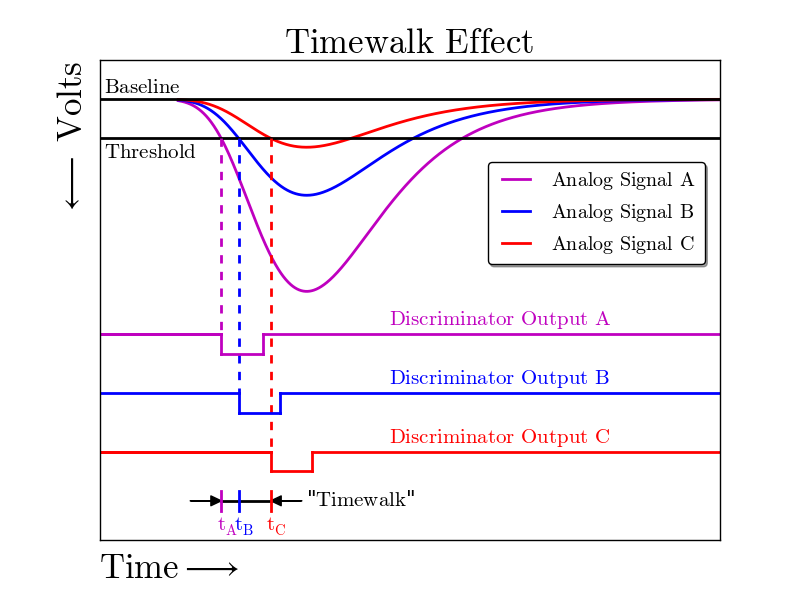
\includegraphics[width=1.0\columnwidth]{calibration/figs/time_walk_effect}
	\caption{Example of the time-walk effect. Three coincident analog signals A, B, \& C of varying amplitudes crossing a fixed threshold in a LED. The discriminator logic output signals vary in time relative to the amplitude of the incoming analog signal.  The signals shown above are simulated analog signals being fed into the LED's thus, they have negative polarity.}
	\label{fig:time_walk_effect}
\end{figure}
As seen in Fig.~\ref{fig:time_walk_effect}, signal A has a larger amplitude as compared to signals B \& C.  It is clear that the logic signal output from the discriminator ``\textit{walks about}'' in time, resulting in an undesirable increase in time resolution of the systems TDC channels.

The time to digital converter (TDC) times reported by the LEDs are subject to the time-walk effect and must be corrected for \textit{via} software so as to optimize the time resolution for each ST channel.  In order to correct the TDC times returned by the F1TDC's one must first acquire a reference time for each hit in the ST, for each event.  